\section{驻点的类型}
\label{sec:saddle-types}

梯度为零的点有哪几类，二阶信息能把它们分开到什么程度？先用一个具体的目标看清这些点的样子，再给定义，然后专门讨论二阶信息判断不了的情形。

\paragraph{贯穿全章的例子}
我们用下面这个目标，它在$x_1$方向是一口双井，在$x_2$方向是一只碗：
\begin{equation}
 f(\bm{x})=\frac14\bigl(x_1^2-1\bigr)^2+\frac12x_2^2.
 \label{eq:saddle-example}
\end{equation}
它的梯度和Hessian可以直接写出：
\begin{equation}
 \nabla f(\bm{x})=\begin{bmatrix}x_1^3-x_1\\x_2\end{bmatrix},\qquad
 \nabla^2 f(\bm{x})=\begin{bmatrix}3x_1^2-1&0\\0&1\end{bmatrix}.
 \label{eq:saddle-example-derivatives}
\end{equation}

令梯度为零，第二个分量给出$x_2=0$，第一个分量给出$x_1(x_1^2-1)=0$。于是有三个驻点，它们的目标值和Hessian是
\[
 \begin{aligned}
 (\pm1,0):&\quad f=0,\quad \nabla^2f=\operatorname{diag}(2,1),\\
 (0,0):&\quad f=\tfrac14,\quad \nabla^2f=\operatorname{diag}(-1,1).
 \end{aligned}
\]

$f\geq0$处处成立，所以$(\pm1,0)$是全局最优解。原点沿$x_2$方向是最低点，沿$x_1$方向是最高点，这正是一个山口。图~\ref{fig:saddle-running-landscape}画出了等高线和$x_2=0$上的截面。

\begin{BookInlineFigure}
  \centering
  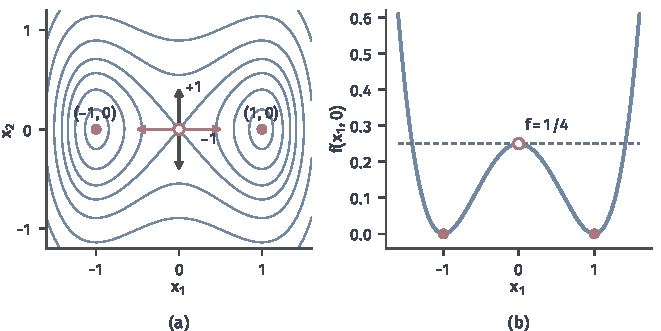
\includegraphics[width=112mm]{figures/05-optimization/02-smooth-optimization/matplotlib/saddle-running-landscape/figure.pdf}
  \caption{目标~\eqref{eq:saddle-example}。(a)蓝线是等高线，红点是两个全局最优解，空心点是原点处的鞍点，红色箭头是曲率为$-1$的方向，灰色箭头是曲率为$+1$的方向。(b)$x_2=0$上的截面，鞍点位于两口井之间的高处，函数值为$1/4$。}
  \label{fig:saddle-running-landscape}
\end{BookInlineFigure}

后面的分析要用到两个常数。Hessian~\eqref{eq:saddle-example-derivatives}的元素随$x_1$增长，全局的常数不存在，所以我们只在带形区域上讨论：
\[
 \bm{U}=\bigl\{\bm{x}\in\mathbb{R}^2:\ \lvert x_1\rvert\leq1\bigr\}.
\]

在$\bm{U}$上，$3x_1^2-1$介于$-1$与$2$之间，因此谱范数$\lVert\nabla^2f\rVert_2\leq2$，光滑常数取$L=2$。Hessian本身的变化由差值控制：
\[
 \bigl\lvert(3x_1^2-1)-(3y_1^2-1)\bigr\rvert
 =3\lvert x_1+y_1\rvert\,\lvert x_1-y_1\rvert
 \leq6\lvert x_1-y_1\rvert.
\]
所以在$\bm{U}$上，Hessian满足下面的Lipschitz条件，常数$M=6$：
\[
 \bigl\lVert\nabla^2f(\bm{x})-\nabla^2f(\bm{y})\bigr\rVert_2\leq M\lVert\bm{x}-\bm{y}\rVert_2.
\]
全章固定步长取$\alpha=1/L=1/2$。

\paragraph{三类驻点}
站在驻点上，一阶变化消失了，目标的走势由Hessian决定。由Taylor公式，对小的$\bm{h}$，
\[
 f(\bm{x}+\bm{h})-f(\bm{x})=\frac12\bm{h}^\top\nabla^2f(\bm{x})\bm{h}+o\bigl(\lVert\bm{h}\rVert_2^2\bigr).
\]
量$\bm{h}^\top\nabla^2f(\bm{x})\bm{h}$的符号回答了“沿这个方向向上弯还是向下弯”。按照能否找到向下弯的方向，驻点分成下面几类。

\begin{definition}[驻点的类型]
 \label{def:saddle-stationary}
 设$f$二阶连续可微。若点$\bm{x}$满足
 \begin{equation}
  \nabla f(\bm{x})=\bm{0},
  \label{eq:saddle-first-order}
 \end{equation}
 就称它为\term{一阶驻点}（first-order stationary point）。若还满足
 \begin{equation}
  \nabla^2f(\bm{x})\succeq\bm{0},
  \label{eq:saddle-second-order}
 \end{equation}
 就称它为\term{二阶驻点}（second-order stationary point）。若一阶驻点满足
 \begin{equation}
  \lambda_{\min}\bigl(\nabla^2f(\bm{x})\bigr)<0,
  \label{eq:saddle-strict}
 \end{equation}
 就称它为\term{严格鞍点}（strict saddle point）。
\end{definition}

一阶驻点要么是二阶驻点，要么是严格鞍点，两者互斥。名称上有一点需要留意：局部极大点也满足式~\eqref{eq:saddle-strict}，在这个约定下同样算作严格鞍点。原因是算法只关心有没有向下弯的方向，而局部极大点和山口在这一点上没有区别。

二阶条件告诉我们这些类别和局部极小点的关系。第~\ref{chap:optimization}章证明过：局部极小点必须是二阶驻点；Hessian正定的一阶驻点一定是严格局部极小点。因此严格鞍点一定不是局部极小点，而二阶驻点之中，Hessian正定的部分一定是局部极小点。

表~\ref{tab:saddle-origin-types}列出几个函数在原点的情形，它们的梯度在原点都为零。前两行是这两条结论直接判定的情形，后三行的Hessian半正定且奇异，正是二阶条件留下的缺口。

\begin{BookInlineTable}
  \centering
  \begin{tabular}{@{}lll@{}}
    \toprule
    函数 & 原点的Hessian & 原点的类型\\
    \midrule
    $x_1^2+x_2^2$ & $\operatorname{diag}(2,2)$ & 严格局部极小点\\
    $x_1^2-x_2^2$ & $\operatorname{diag}(2,-2)$ & 严格鞍点\\
    $x_1^2+x_2^4$ & $\operatorname{diag}(2,0)$ & 二阶驻点，局部极小点\\
    $x_1^2-x_2^4$ & $\operatorname{diag}(2,0)$ & 二阶驻点，不是局部极小点\\
    $x_1^4-x_2^4$ & $\bm{0}$ & 二阶驻点，不是局部极小点\\
    \bottomrule
  \end{tabular}
  \caption{原点处的几种情形。第三行与第四行的梯度和Hessian完全相同，类型却不同。}
  \label{tab:saddle-origin-types}
\end{BookInlineTable}

\paragraph{退化情形}
Hessian半正定仍不足以说明是局部极小点。比较$x_1^2+x_2^4$和$x_1^2-x_2^4$：它们在原点的函数值、梯度和Hessian完全一样，差别只在四阶项。沿$x_2$轴看，
\[
 x_1^2+x_2^4\big|_{x_1=0}=t^4,\qquad
 x_1^2-x_2^4\big|_{x_1=0}=-t^4.
\]

前者把原点托在最低处，后者从原点沿$x_2$轴一直下降。只看到二阶为止的信息，这两个函数无法分开。图~\ref{fig:saddle-stationary-zoo}用浅红色标出比原点函数值更低的区域，只要原点的任意小邻域内有浅红色，原点就不是局部极小点。

\begin{BookInlineFigure}
  \centering
  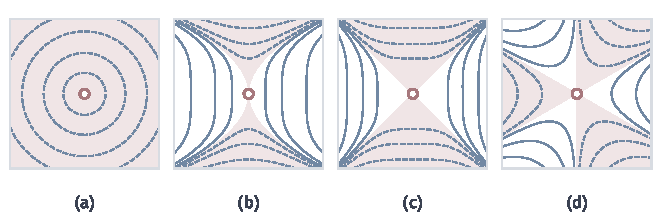
\includegraphics[width=112mm]{figures/05-optimization/02-smooth-optimization/matplotlib/saddle-stationary-zoo/figure.pdf}
  \caption{原点处四种不是局部极小点的驻点，蓝线是等高线，虚线为负值，浅红区域是函数值低于$f(\bm{0})=0$的点。(a)$-x_1^2-x_2^2$，局部极大点。(b)$x_1^2-x_2^4$，Hessian为$\operatorname{diag}(2,0)$。(c)$x_1^4-x_2^4$，Hessian为零。(d)$x_1^3-3x_1x_2^2$，Hessian为零。后三个都没有负曲率，算法靠Hessian察觉不到下降方向。}
  \label{fig:saddle-stationary-zoo}
\end{BookInlineFigure}

图中(a)的负曲率是显式的，(b)、(c)、(d)的下降则藏在更高阶的项里。(d)沿$x_1$轴的函数值是$t^3$，经过原点时由正变负，下降的一侧和上升的一侧挨在一起。

\paragraph{每条直线上都最低，仍然不是局部极小}
有人会想：既然二阶信息只看直线方向，那么补上高阶项，逐条直线检查目标是否在原点取到局部最低，总该够了吧？下面的例子说明还是不够：
\begin{equation}
 f(\bm{x})=\bigl(x_2-x_1^2\bigr)\bigl(x_2-2x_1^2\bigr).
 \label{eq:saddle-peano}
\end{equation}

展开得到$x_2^2-3x_1^2x_2+2x_1^4$，所以原点是驻点，Hessian是$\operatorname{diag}(0,2)$。先看经过原点的每条直线。沿$x_2=mx_1$，目标是
\[
 f(t,mt)=m^2t^2-3mt^3+2t^4.
\]

$m\neq0$时二次项为正，$t$足够小时函数值为正。$m=0$时是$2t^4$，沿$x_2$轴是$x_2^2$，也都大于零。所以原点在每条直线上都是严格局部最低点。

可是沿抛物线$x_2=\tfrac32x_1^2$走，两个因子一正一负：
\[
 f\bigl(t,\tfrac32t^2\bigr)=\Bigl(\tfrac12t^2\Bigr)\Bigl(-\tfrac12t^2\Bigr)=-\frac14t^4<0.
\]

原点的任意小邻域内都有比它更低的点，所以它不是局部极小点。图~\ref{fig:saddle-peano}(a)给出了几何解释：函数值为负的区域夹在两条抛物线之间，而任何一条直线在原点附近都会离开这个弯曲的窄缝。沿直线下降的想法，在这里看不到弯曲的下降路径。

\begin{BookInlineFigure}
  \centering
  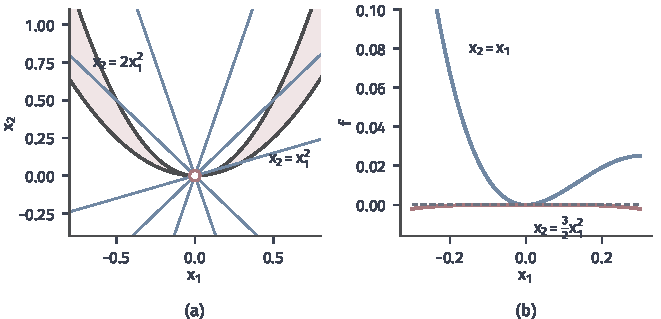
\includegraphics[width=112mm]{figures/05-optimization/02-smooth-optimization/matplotlib/saddle-peano/figure.pdf}
  \caption{目标~\eqref{eq:saddle-peano}。(a)浅红色是$f<0$的区域，夹在抛物线$x_2=x_1^2$和$x_2=2x_1^2$之间；蓝色直线在原点附近都位于这个区域之外。(b)沿直线$x_2=x_1$的函数值（蓝）在原点取最低，沿抛物线$x_2=\tfrac32x_1^2$的函数值（红）为负。}
  \label{fig:saddle-peano}
\end{BookInlineFigure}

\paragraph{二阶条件能排除什么}
把这些类别按包含关系排列，得到图~\ref{fig:saddle-class-nesting}。每往里一层，条件就强一些。

\begin{BookInlineFigure}
  \centering
  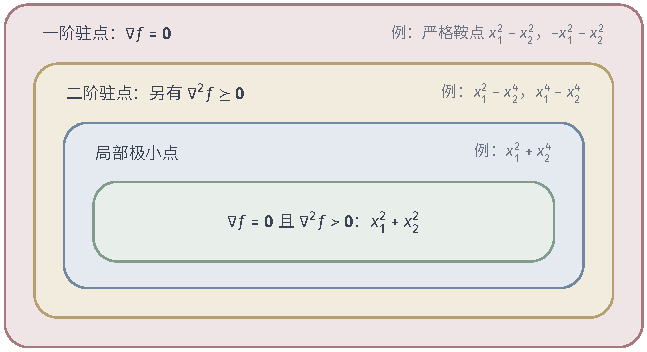
\includegraphics[width=109.6mm]{figures/05-optimization/02-smooth-optimization/tikz/saddle-class-nesting/figure.pdf}
  \caption{驻点类别的包含关系，每层右上角的函数在原点属于该层而不属于更内一层。最外层与第二层之间的差就是严格鞍点。第二层与第三层之间是退化的二阶驻点，二阶信息无法把它们和局部极小点分开。}
  \label{fig:saddle-class-nesting}
\end{BookInlineFigure}

由此可以说清楚二阶信息的能力。负特征值是确凿的证据：只要算出一个负的曲率，就能断定这里不是局部极小点。Hessian正定也是确凿的证据：这里一定是严格局部极小点。两者之间的情形，二阶信息保持沉默，并不是“大概是极小点”的意思。

所以算法的目标要说得克制。排除严格鞍点是可以做到的事，这是后面几节的内容。判定一个退化的二阶驻点是否为局部极小点，一般需要更高阶的信息，本章的方法不处理。

\paragraph{局部条件不说明全局}
上面的讨论还停留在局部。即使某点确实是局部极小点，也不说明它是全局最优解。看下面这个倾斜的双井：
\[
 \psi(x)=\frac14x^4+\frac13x^3-x^2,\qquad
 \psi'(x)=x(x-1)(x+2).
\]

三个驻点的二阶导数由$\psi''(x)=3x^2+2x-2$算出：
\[
 \psi''(0)=-2,\qquad\psi''(1)=3,\qquad\psi''(-2)=6.
\]

$x=1$是严格局部极小点，满足所有局部条件，函数值却是$-5/12$，而全局最优解$x=-2$的函数值是$-8/3$。图~\ref{fig:saddle-tilted-well}中，从$x=1$到更低的井要先翻过$x=0$处的高坡。站在黄点上，任何只依赖当地导数的判据都看不到另一口井。

\begin{BookInlineFigure}
  \centering
  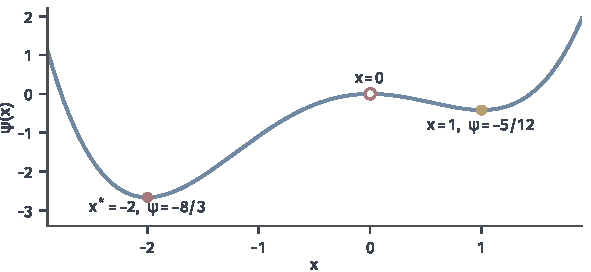
\includegraphics[width=100mm]{figures/05-optimization/02-smooth-optimization/matplotlib/saddle-tilted-well/figure.pdf}
  \caption{倾斜双井$\psi(x)=x^4/4+x^3/3-x^2$。黄点$x=1$是严格局部极小点，红点$x=-2$是全局最优解，空心点$x=0$是局部极大点。局部条件在黄点全部满足。}
  \label{fig:saddle-tilted-well}
\end{BookInlineFigure}

所以本章的“离开鞍点”只是把严格鞍点从可能的终点中排除。它既不判定退化的二阶驻点，也不保证到达全局最优解。

